\section{Cycle-Jump Demonstration Using a Chaboche Unified Viscoplastic UMAT}

\subsection{Motivation}

Long cyclic simulations are computationally expensive when every loading cycle is resolved explicitly. A cycle-jump approach reduces the cost by identifying a stabilized per-cycle evolution of selected internal variables and extrapolating this evolution over many cycles. In the present demonstration, the cycle-jump variable is the accumulated viscoplastic strain stored by the UMAT as SDV1.

\subsection{Abaqus--UMAT Model}

The model was implemented in Abaqus/Standard using a single C3D8 block element smoke-test geometry. The material response was described by a Chaboche-v1 unified viscoplastic UMAT and loaded under displacement-controlled fully reversed cyclic loading. The state variable SDV1 represents the accumulated viscoplastic strain \(p\), while SDV15 stores the last viscoplastic increment. This compact setup was selected to isolate the UMAT response, the Abaqus interface, and the cycle-jump postprocessing workflow.

\begin{figure}[htbp]
    \centering
    
\includegraphics[width=0.92\textwidth]{figures/fig00_geometry_material_model.png}
    \caption{Single-element Abaqus validation model and Chaboche-v1 material-state workflow. The block is a one-element C3D8 specimen with \(L_0=10~\mathrm{mm}\), a \(2~\mathrm{mm}\times2~\mathrm{mm}\) cross-section, fixed left face, and displacement-controlled cyclic loading on the right face.}
    \label{fig:geometry_material_model}
\end{figure}

\begin{figure}[htbp]
    \centering
    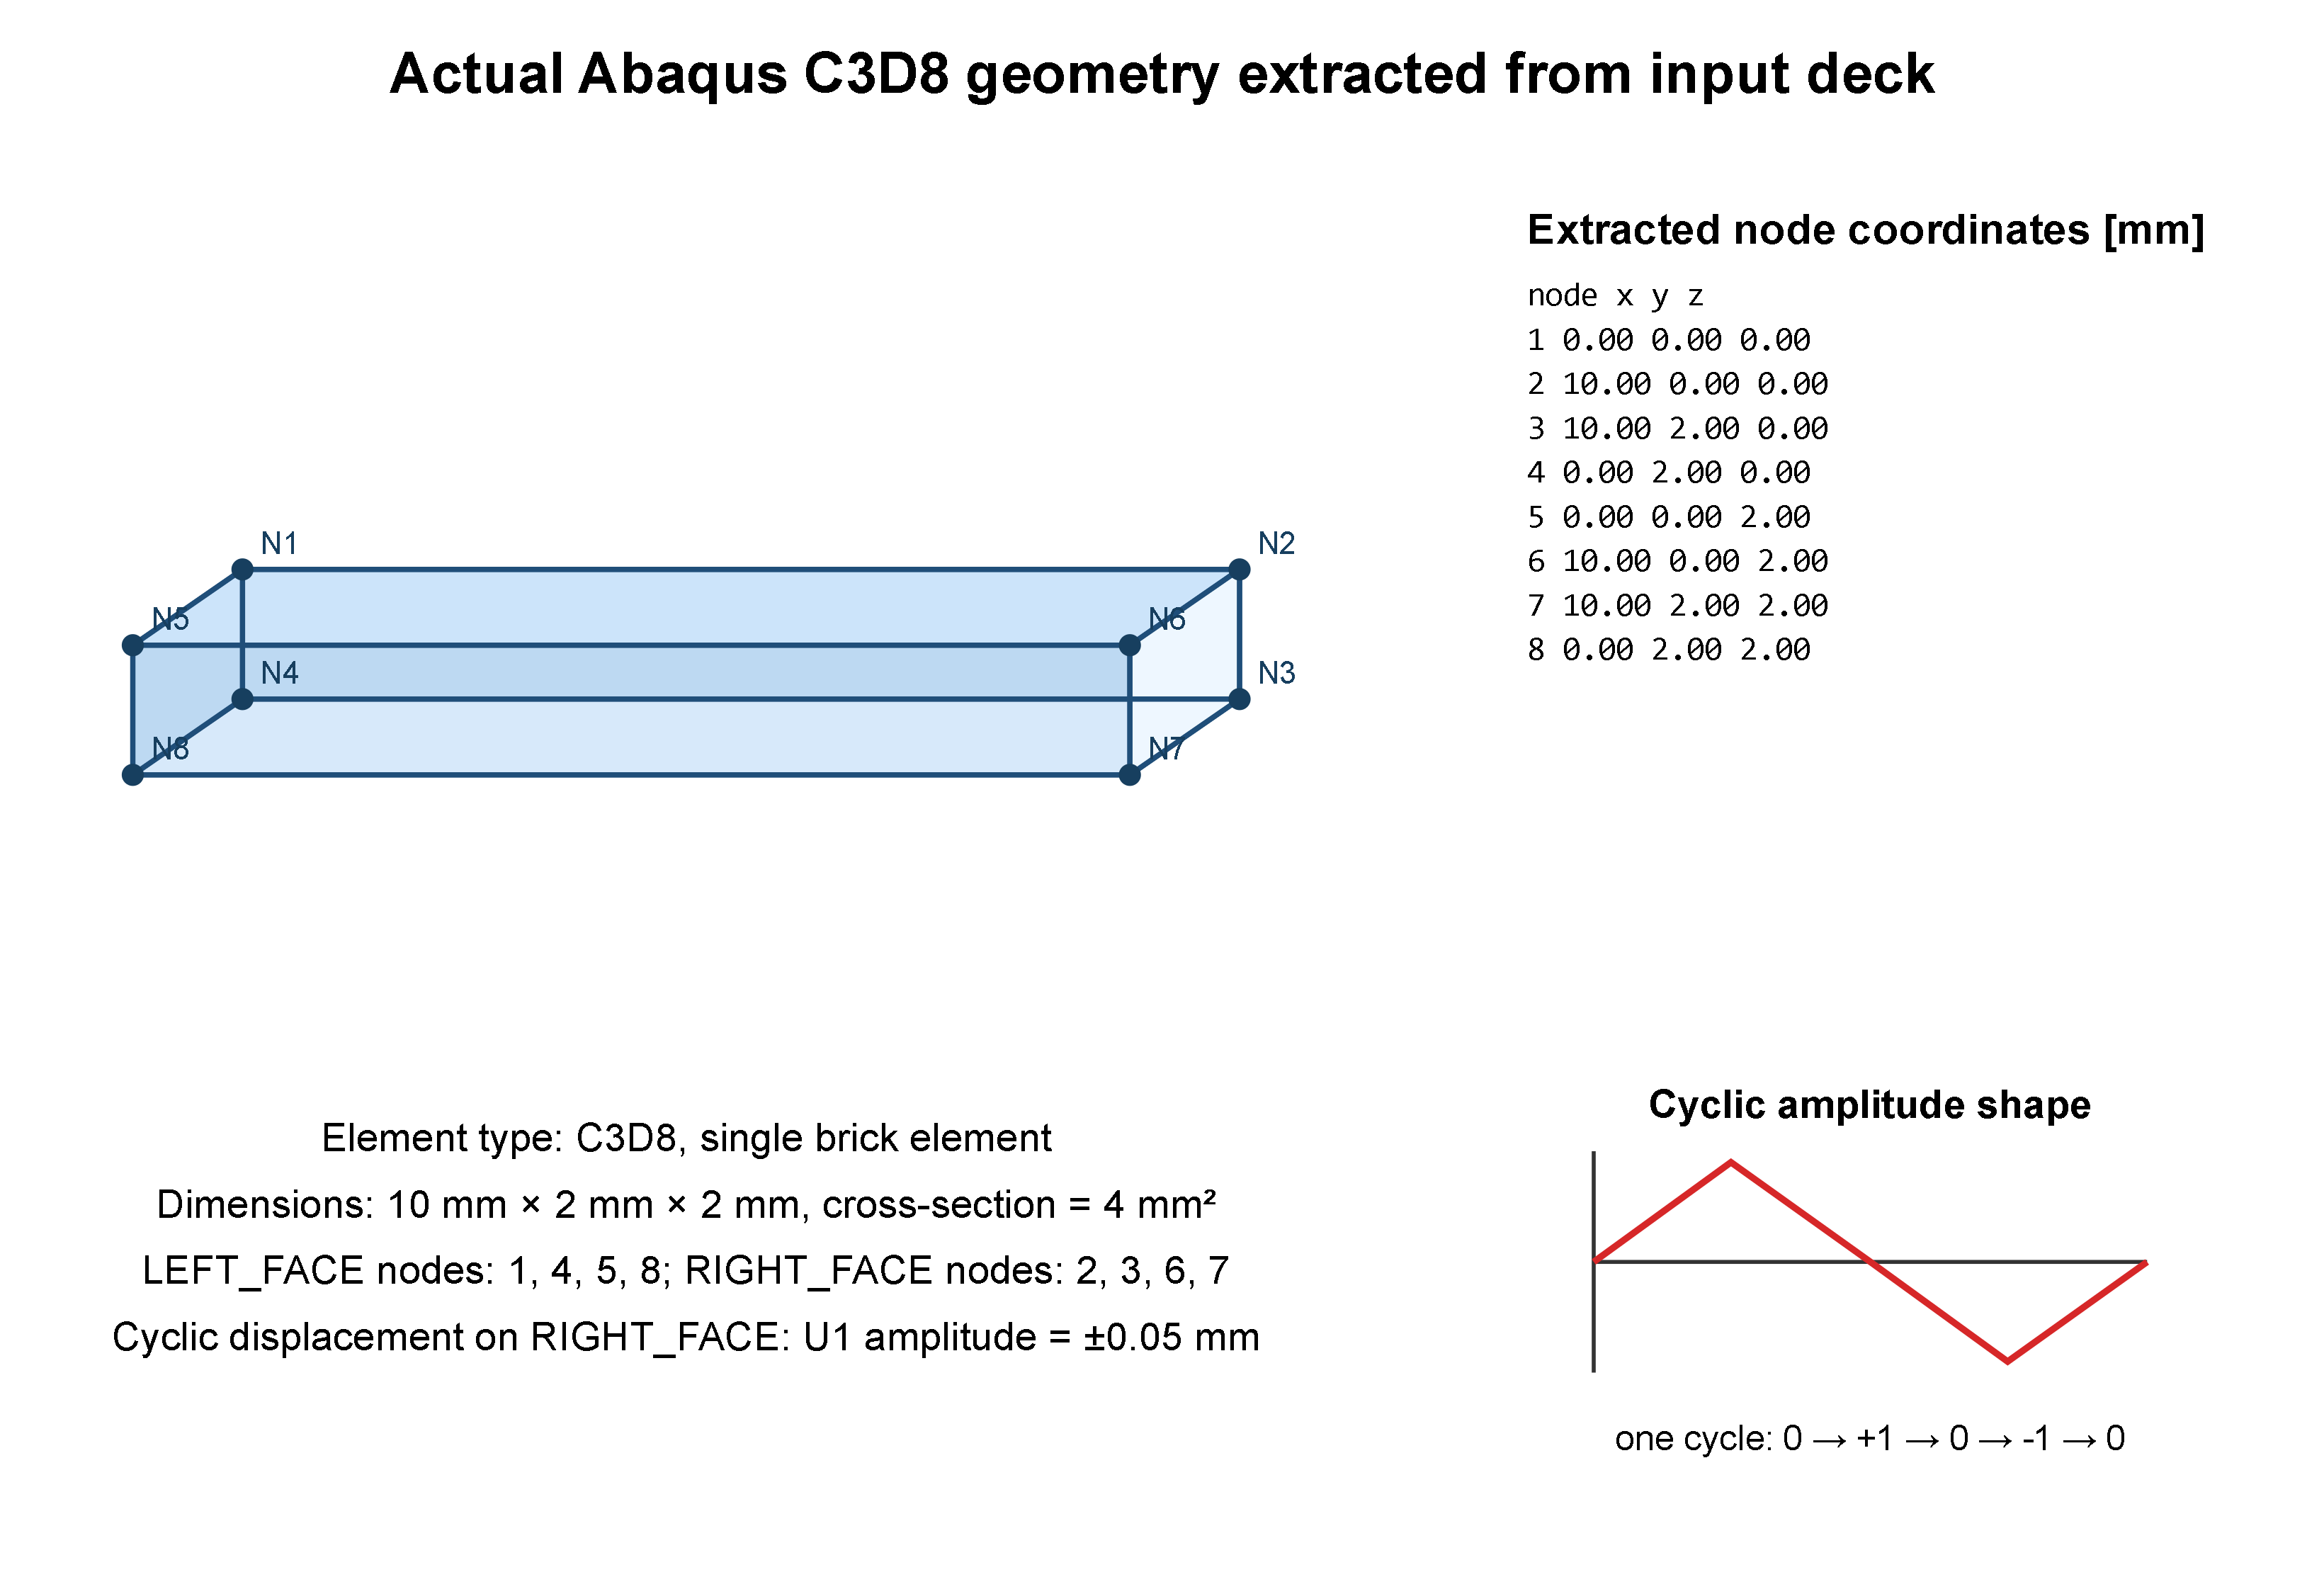
\includegraphics[width=0.92\textwidth]{figures/fig00b_actual_abaqus_geometry.png}
    \caption{Actual Abaqus single-element geometry reconstructed from the input deck using the node coordinates and C3D8 element connectivity. The extracted model confirms the \(10~\mathrm{mm}\times2~\mathrm{mm}\times2~\mathrm{mm}\) block, the left and right node sets, and the displacement-controlled cyclic loading direction.}
    \label{fig:actual_abaqus_geometry}
\end{figure}

\subsection{Amplitude Selection}

An amplitude sweep was first performed to identify a physically useful validation amplitude. The \(\pm0.1\%\) and \(\pm0.2\%\) cases remained elastic or near-elastic, whereas the \(\pm0.5\%\) case activated viscoplasticity at a moderate stress level. The \(\pm1.0\%\) case produced stronger plastic cycling. Therefore, the \(\pm0.5\%\) strain amplitude was selected for the cycle-jump demonstration.

\begin{figure}[htbp]
    \centering
    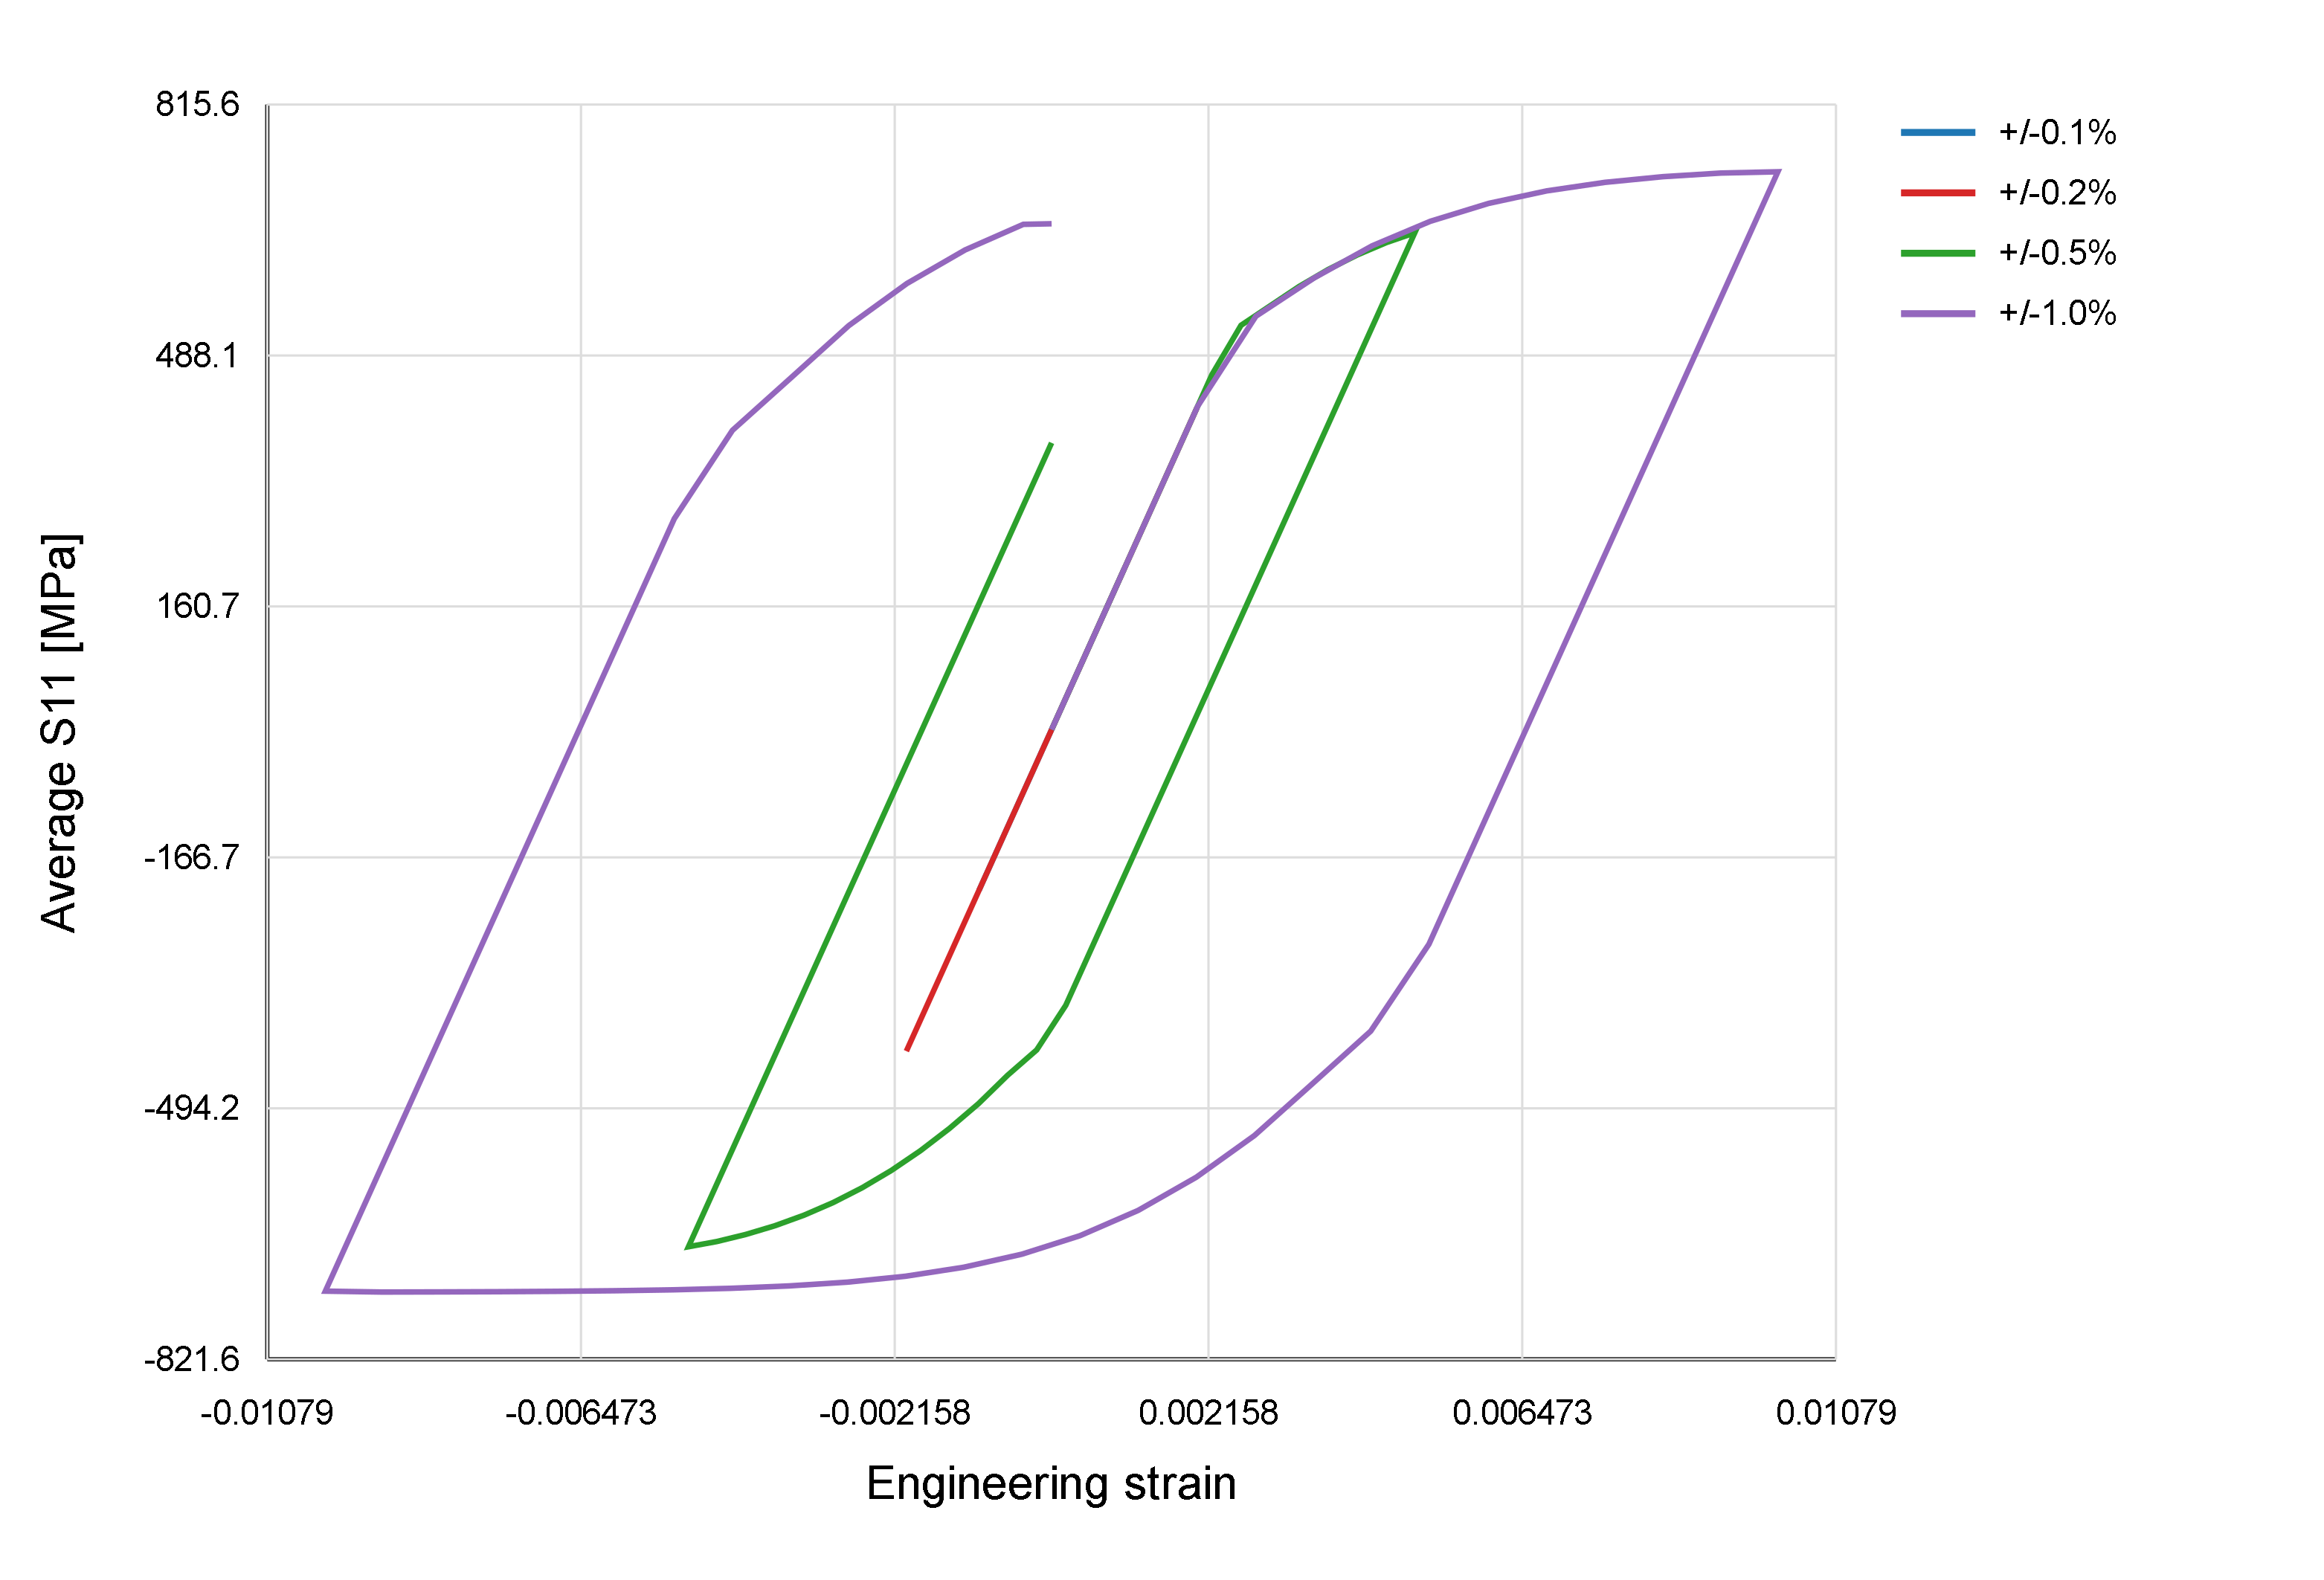
\includegraphics[width=0.82\textwidth]{figures/fig01_amplitude_sweep_stress_strain.png}
    \caption{Amplitude sweep for the Chaboche-v1 UMAT. The smaller amplitudes remain mainly elastic, while the $\pm0.5\%$ case activates viscoplasticity at a moderate stress level and was selected for the cycle-jump demonstration.}
    \label{fig:amplitude_sweep}
\end{figure}

\subsection{Explicit 10-Cycle Baseline}

The selected \(\pm0.5\%\) case was simulated explicitly for 10 cycles. The analysis completed with 507 increments, 0 cutbacks, 0 warnings, and 0 errors. The simulation produced nonzero stress, nonzero reaction force, and monotonic accumulated state-variable evolution. The selected hysteresis loops show that the loop shape becomes nearly repeatable after the first-cycle transient.

\begin{figure}[htbp]
    \centering
    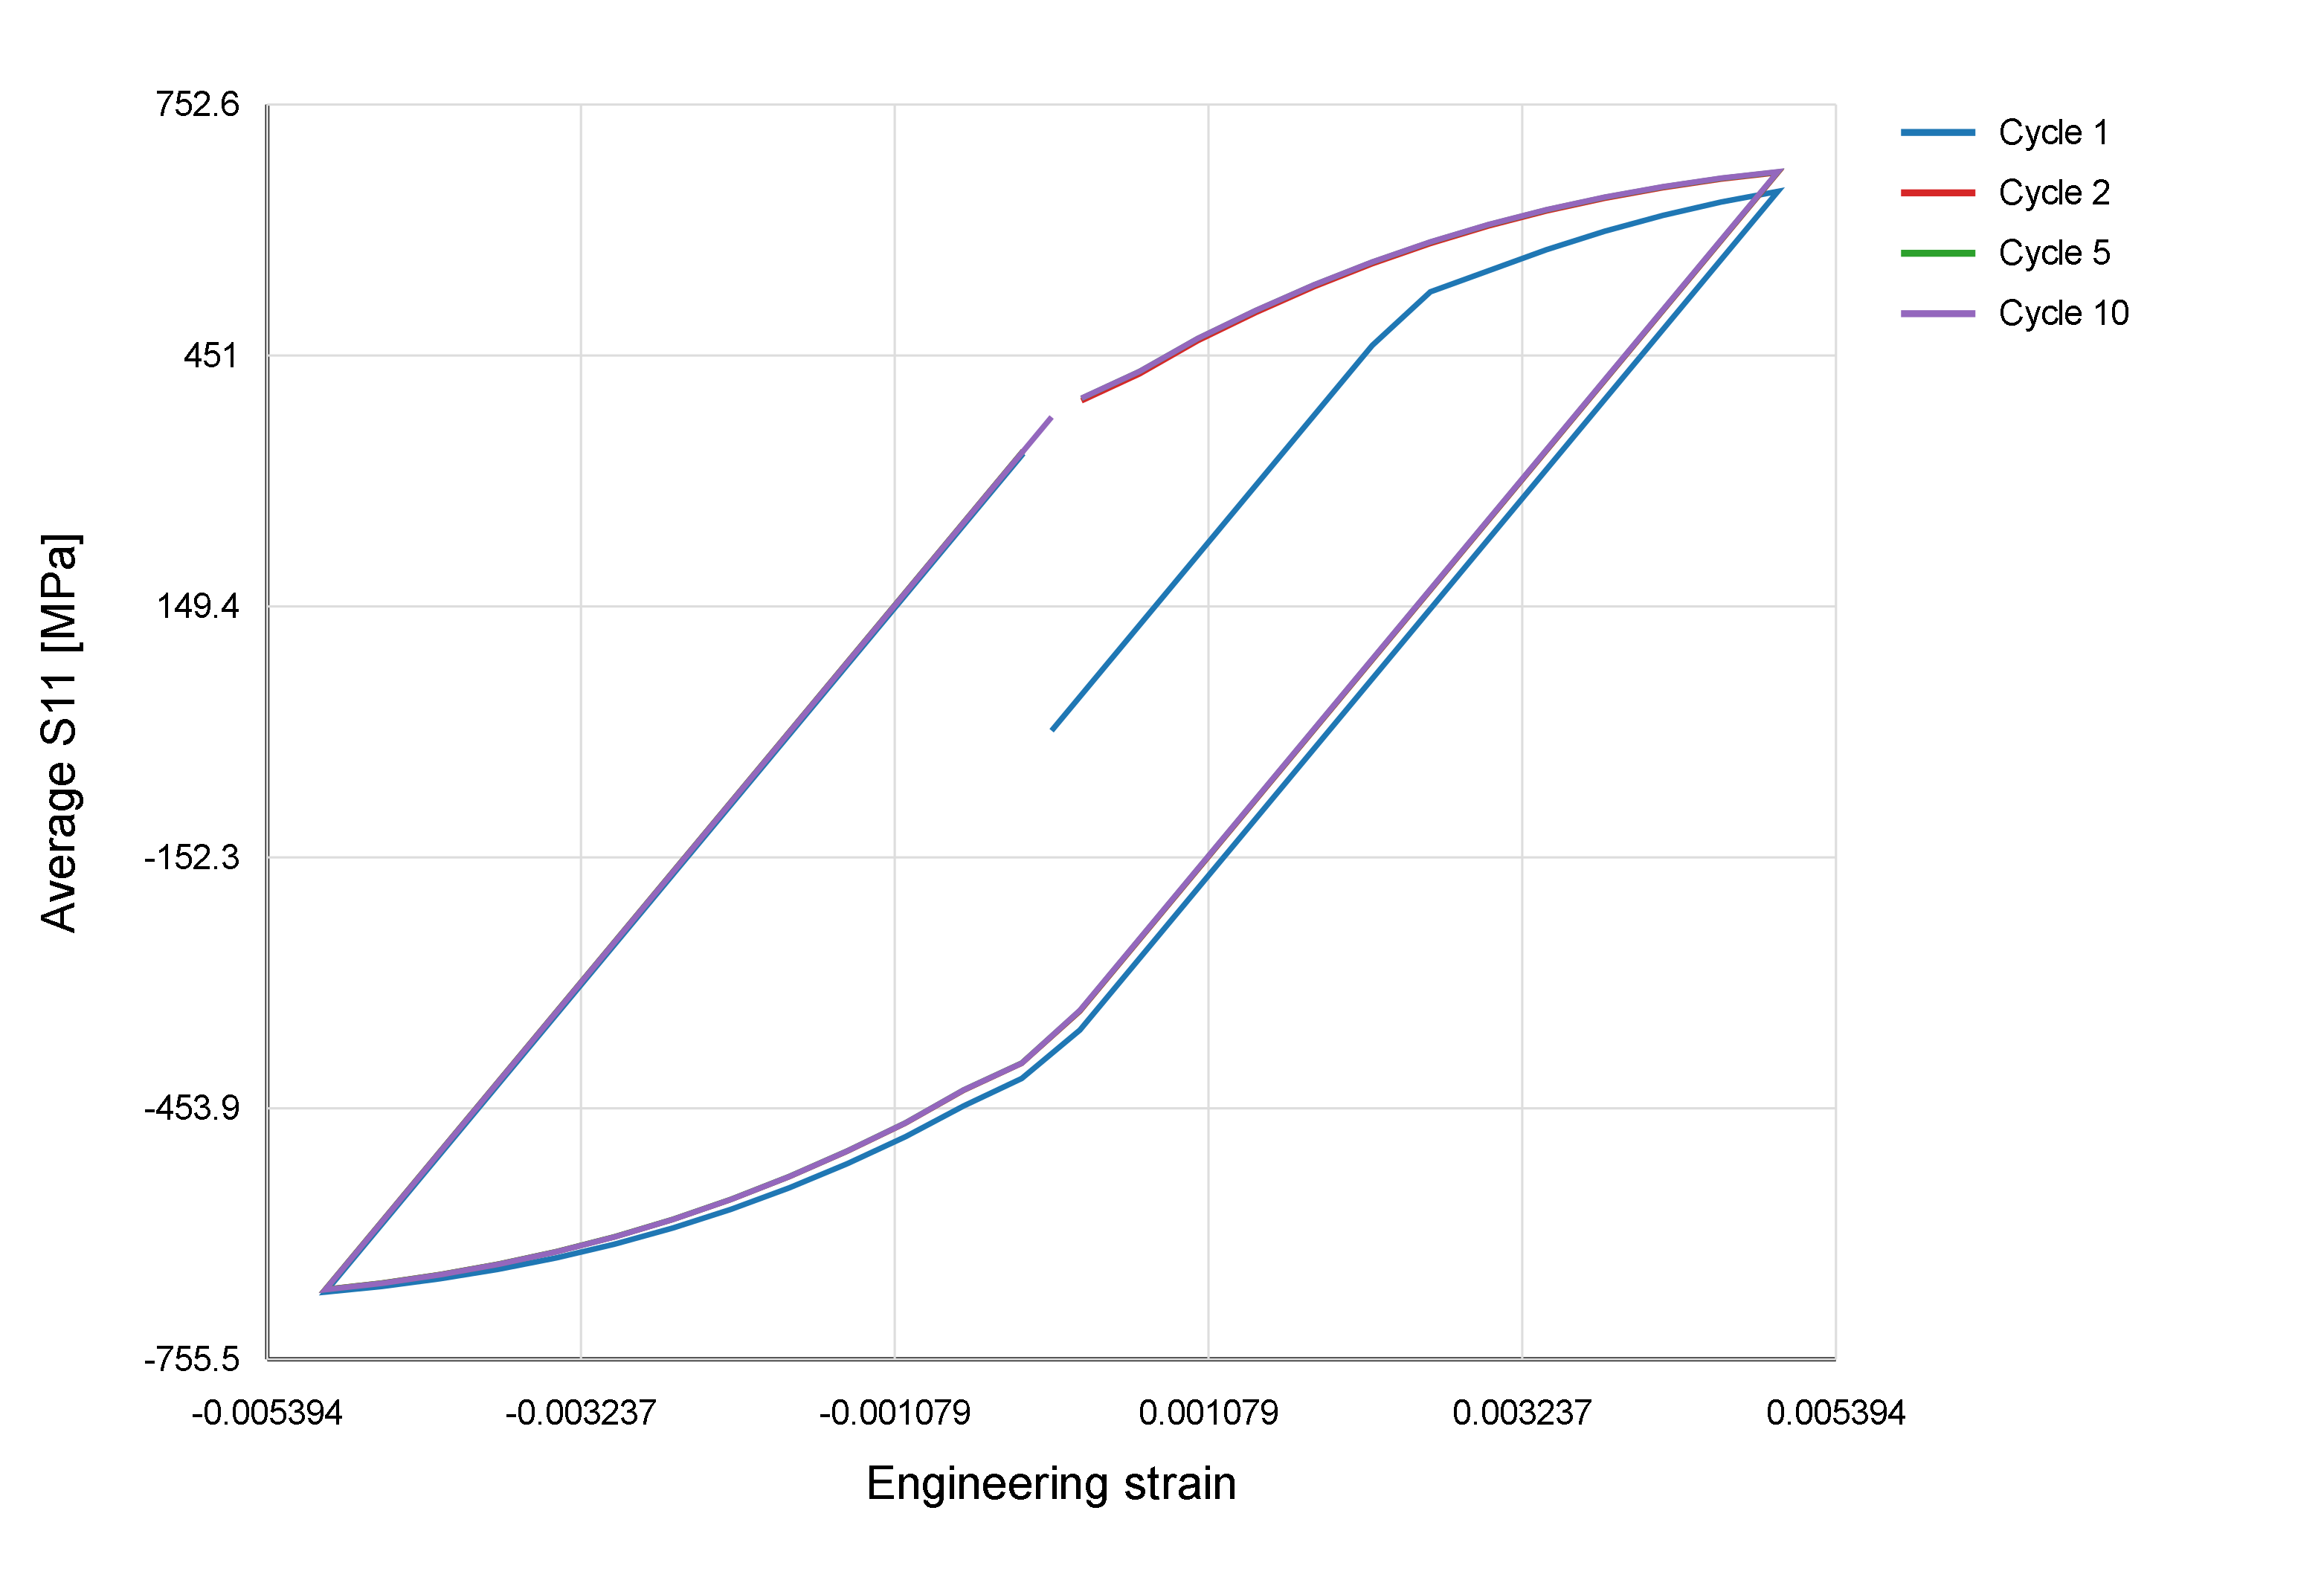
\includegraphics[width=0.82\textwidth]{figures/fig02_10cycle_selected_hysteresis_loops.png}
    \caption{Selected hysteresis loops from the explicit 10-cycle Abaqus simulation at $\pm0.5\%$ strain amplitude. The loop shape becomes nearly repeatable after the initial transient.}
    \label{fig:ten_cycle_loops}
\end{figure}

\subsection{Stabilized Internal-Variable Increment}

The total SDV1 value is cumulative because it represents accumulated viscoplastic strain. It should therefore increase monotonically and should not be used directly as a stabilization criterion. Instead, stabilization was assessed using the per-cycle increment \(\Delta\mathrm{SDV1}\). Cycles 2--10 were used as the stabilized reference window. Over this window, the mean increment was \(0.007185465191\), the standard deviation was \(3.368213202\times10^{-6}\), and the relative range was \(0.001429037192\), corresponding to approximately \(0.1429\%\).

\begin{figure}[htbp]
    \centering
    
\includegraphics[width=0.82\textwidth]{figures/fig03_delta_sdv1_per_cycle.png}
    \caption{Per-cycle increment of accumulated viscoplastic strain. After the first cycle, the increment remains nearly constant, supporting the use of a cycle-jump predictor.}
    \label{fig:delta_sdv1}
\end{figure}

\subsection{Cycle-Jump Predictor}

The postprocessing-level cycle-jump predictor was defined as

\[
p_N^{\mathrm{pred}} =
p_{10} + (N-10)\,\overline{\Delta p}_{2-10},
\]

where \(p_N^{\mathrm{pred}}\) is the predicted accumulated viscoplastic strain at cycle \(N\), \(p_{10}\) is the explicit value at cycle 10, and \(\overline{\Delta p}_{2-10}\) is the mean per-cycle increment from cycles 2--10. The resulting predictions were \(p_{20}=0.1421214351\), \(p_{50}=0.3576853909\), \(p_{100}=0.7169586504\), \(p_{200}=1.435505169\), \(p_{500}=3.591144727\), and \(p_{1000}=7.183877322\).

\begin{figure}[htbp]
    \centering
    
\includegraphics[width=0.82\textwidth]{figures/fig04_cycle_jump_sdv1_prediction.png}
    \caption{Cycle-jump prediction of accumulated viscoplastic strain using the stabilized per-cycle increment obtained from explicit cycles 2--10.}
    \label{fig:jump_prediction}
\end{figure}

\subsection{Explicit 20-Cycle Validation}

A separate explicit 20-cycle Abaqus simulation was performed to validate the cycle-jump prediction. This analysis completed with 1007 increments, 0 cutbacks, 0 warnings, and 0 errors. The predicted SDV1 value at cycle 20 was 0.1421214351, while the explicit Abaqus result was 0.1420256943. The absolute error was \(-9.574084894\times10^{-5}\), corresponding to a relative error of 0.0674\%.

\begin{figure}[htbp]
    \centering
    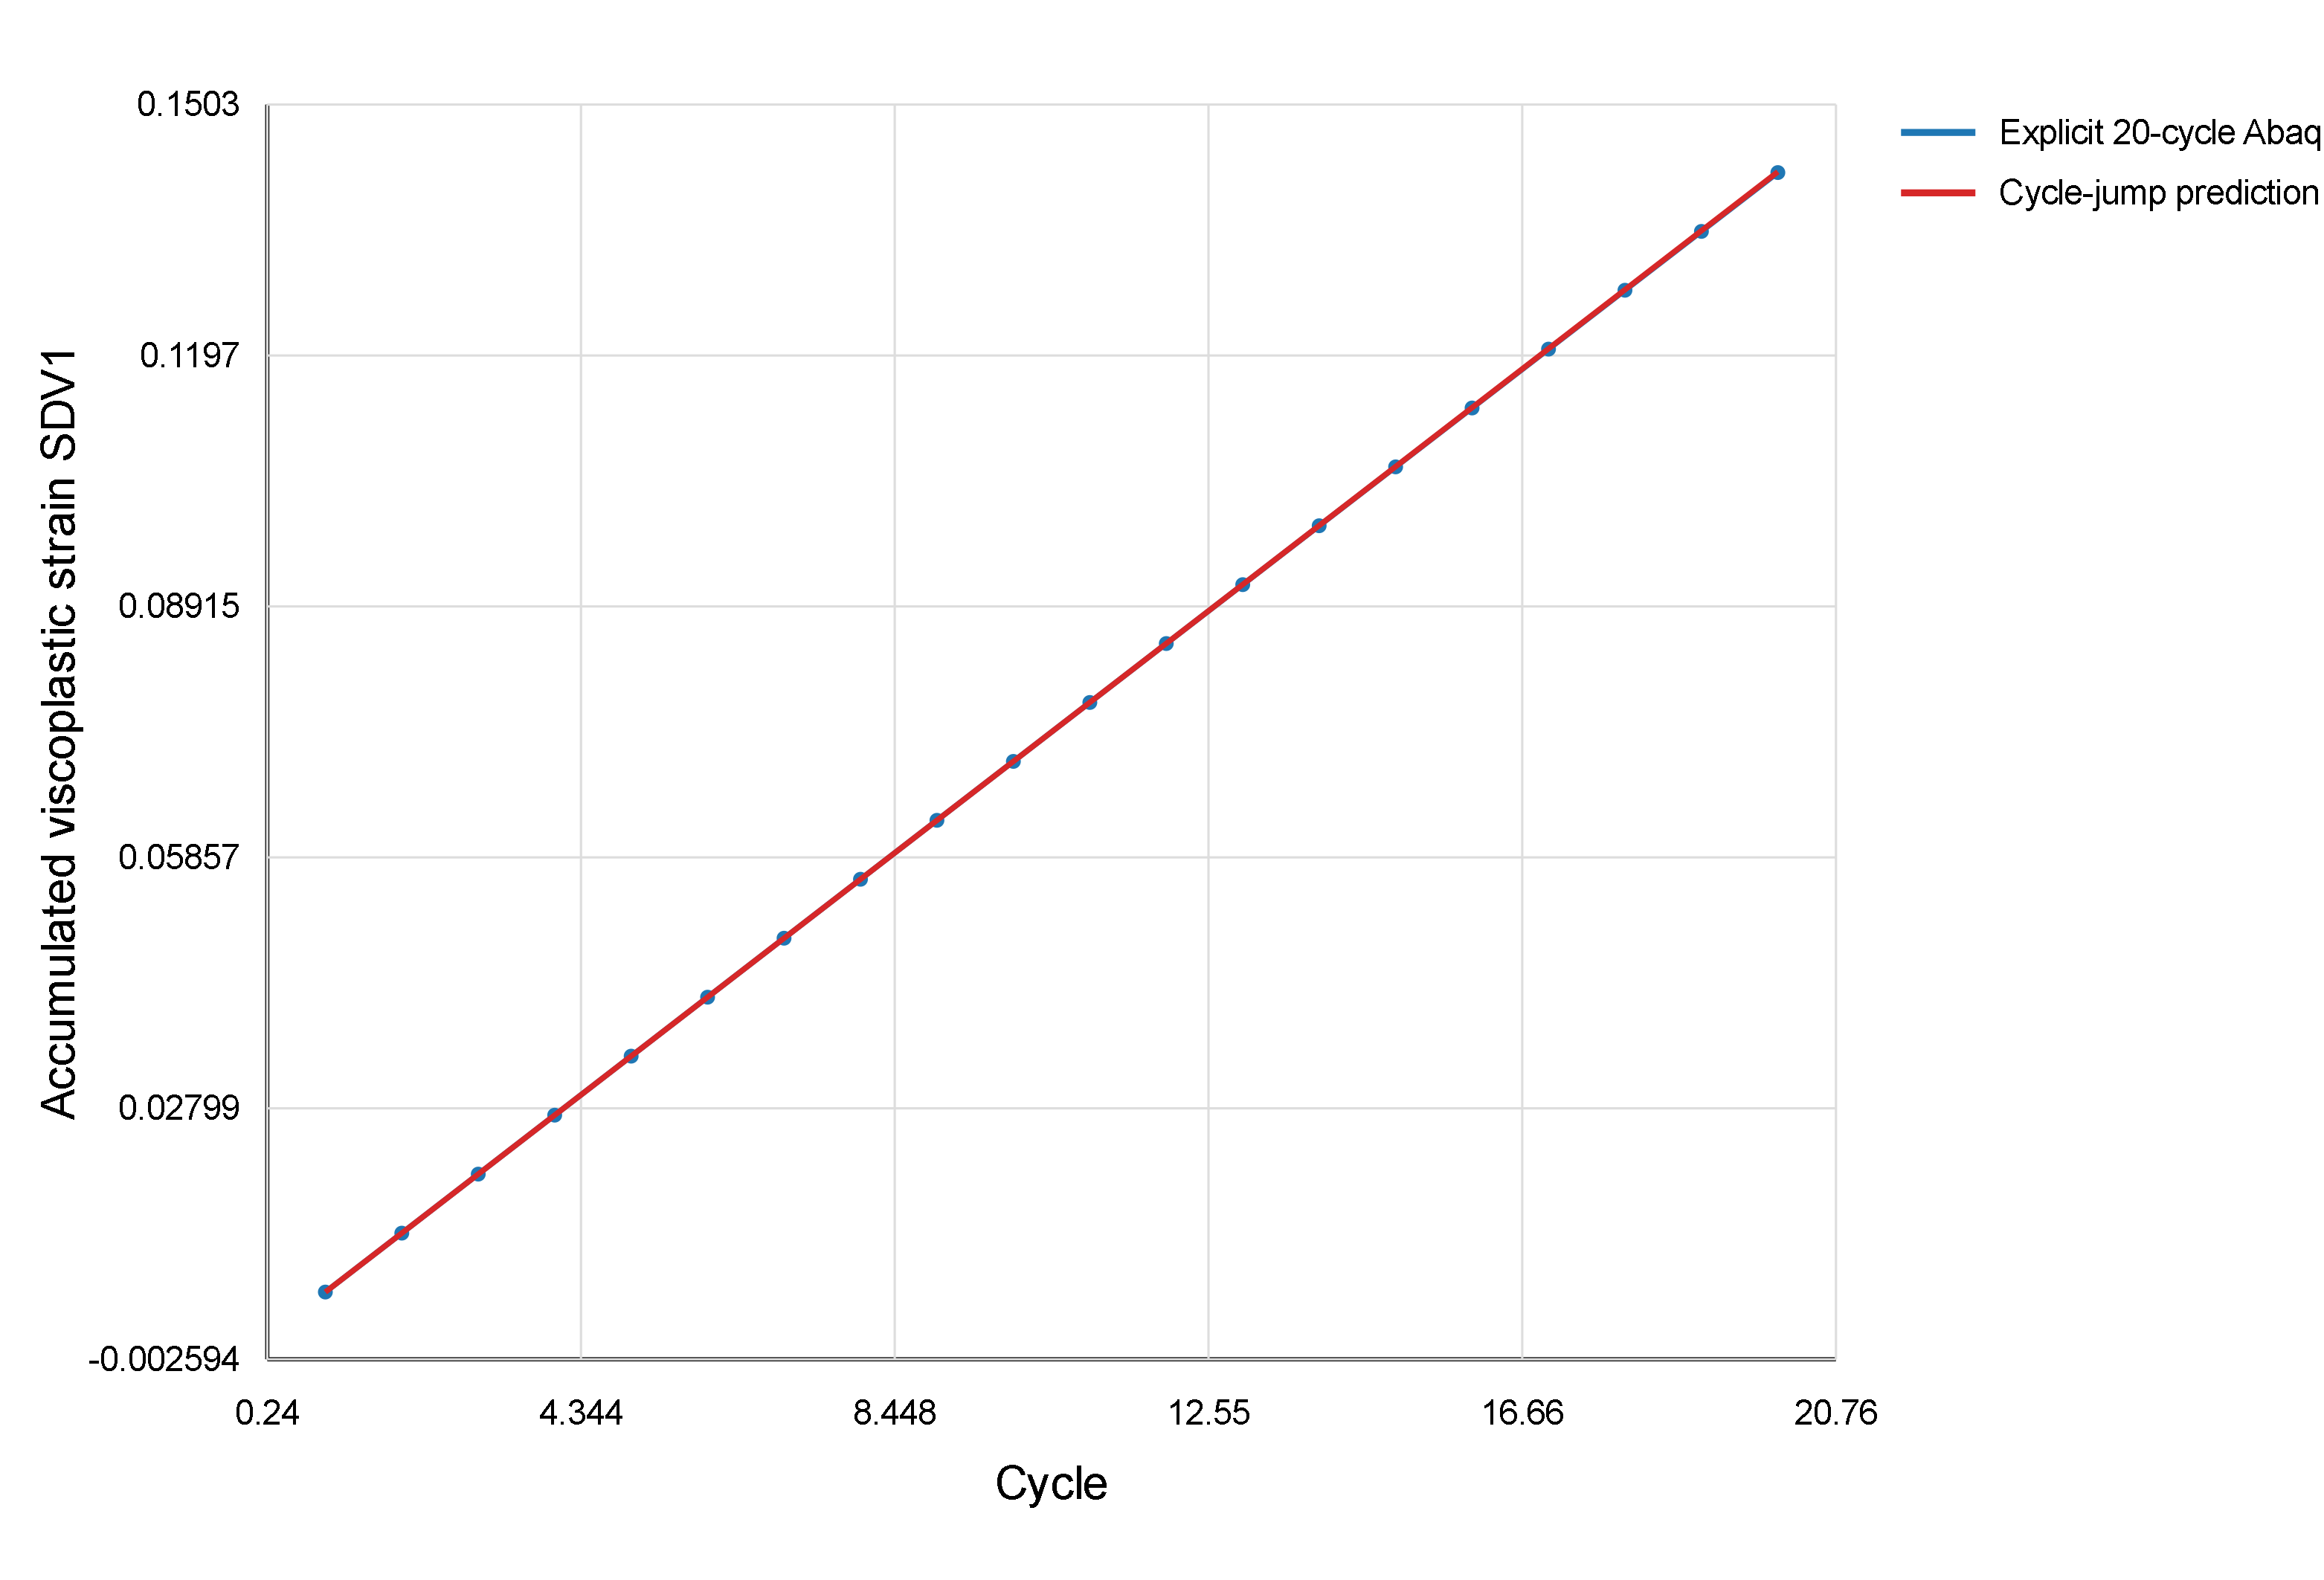
\includegraphics[width=0.82\textwidth]{figures/fig05_cycle_jump_vs_explicit_20cycles.png}
    \caption{Validation of the cycle-jump predictor against an independent explicit 20-cycle Abaqus simulation. The predicted and explicit SDV1 values agree closely, with a relative error of 0.0674\% at cycle 20.}
    \label{fig:jump_validation}
\end{figure}

\subsection{Discussion and Limitations}

This result validates a postprocessing-level cycle-jump predictor for the simplified Chaboche-v1 model and the selected \(\pm0.5\%\) strain-amplitude test case. The method does not yet inject jumped STATEV values into Abaqus and is not yet a calibrated fatigue-life model. The next implementation step would be state-variable injection using SDVINI, restart analysis, or another Abaqus workflow that initializes the material state after a cycle jump.

The Chaboche unified viscoplastic UMAT has therefore been successfully implemented and validated at the computational workflow level. It reproduces nonzero stress, reaction force, viscoplastic strain accumulation, cyclic hysteresis, and a stable per-cycle internal-variable increment suitable for cycle-jump prediction. However, the current Chaboche-v1 parameter set should be treated as a demonstration and validation set, not yet as a fully calibrated 316 stainless steel material model.

\subsection{Summary}

The Chaboche-v1 UMAT, cyclic Abaqus workflow, postprocessing scripts, and cycle-jump predictor were validated. Explicit cycles 2--10 provided a stabilized per-cycle increment of accumulated viscoplastic strain, and the explicit 20-cycle check confirmed the prediction accuracy with only 0.0674\% relative error in SDV1 at cycle 20.

